%=========================================================
% cJTAG 
%=========================================================
\section{cJTAG (Compact JTAG)}
\label{sec:cJTAG}

While the debug interface of mmRISC-1 core is essentially 4-wire JTAG, the mmRISC-1 project supports 2-wire cJTAG (Compact JTAG) as its debug interface instead of 4-wire JTAG. This project provides a module CJTAG\_2\_JTAG to convert 2-wire cJTAG to 4-wire JTAG which is located at outside of mmRISC-1 core boundary, that is at chip top layer. If you want to use cJTAG, please enable \textasciigrave define ENABLE\_CJTAG switch in common/defines\_chip.v.\\
The cJTAG interface consists of only TCKC and TMSC as shown in Table \ref{tb:cJTAG_SIGNAL}.\\
The relationship between the frequency of the system clock and TCKC does not matter. For example, both cases with fCLK=20MHZ/fTCK=10MHz and fCLK=100KHz/fTCK=10MHz are OK.

\begin{table}[hbtp]
    \begin{adjustbox}{scale={1.0}{1.0}}
    \textsf{
    \begin{tabular}{lll}
        \hline
        %--------------------------------
        \rowcolor{LightPurple}
        \textbf{Name} &
        \textbf{Meaning} &
        \textbf{Description} \\
        \hline
        %--------------------------------
        TCKC  & Test Clock for cJTAG        & Clock which is driven by external Adapter. \\
        TMSC  & Test Mode Select for cJTAG  & Bi-directional Serial Data  \\
        %--------------------------------
        \hline
    \end{tabular}
    }
    \end{adjustbox}
    \caption{Signal of cJTAG Interface}
    \label{tb:cJTAG_SIGNAL}
\end{table}

%=========================================================
% cJTAG Signal Sequence
%=========================================================
\subsection{cJTAG Signal Sequence}
The cJTAG signal sequence is divided into 3 phases shown below.

\begin{description}

    \item[Escape Sequence]\mbox{}\\
        After the reset, the CJTAG\_2\_JTAG is in Offline state. While TCKC is held high, TMSC is toggled(L\textrightarrow H\textrightarrow L) 3 times or more, the CJTAG\_2\_JTAG detects escape sequence and enters Online state as shown in Figure \ref{fig:cJTAG_ESC_ACT}(a).

    \item[Activation Sequence]\mbox{}\\
        After the Online Sequence, the CJTAG\_2\_JTAG waits for the Activation Sequence as shown in Figure \ref{fig:cJTAG_ESC_ACT}(b). During this sequence, TMSC is driven by external adapter, and the CJTAG\_2\_JTAG samples TMSC at the rising edge of TCKC. If it detects the Activation Sequence for OSCAN1, which consists of (1) OAC (Online Activation Code) = 4'b0011 (MSB first), (2) EC (Extension Code) = 4'b0001, and (3) CP (Check Packet) = 4'b0000, it enters OSCAN1 mode. If it detects any other sequence, it returns to Offline state.       

    \item[OSCAN1 Sequence]\mbox{}\\
        In OSCAN1 mode, the CJTAG\_2\_JTAG starts to convert from cJTAG to JTAG as its essential function. The JTAG source signals TMS, TDI and TDO are multiplexed onto the the TMSC signal, and three TCKC rising edges are required to perform one bit of JTAG scan as shown in Figure \ref{fig:cJTAG_OSCAN1}. At the first rising edge of TCKC, TMSC is driven by an external adapter and conveys the inverse of TDI. At the second rising edge of TCKC, TMSC is driven by an external adapter and conveys TMS. And at the third rising edge of TCKC, TMSC is driven by the CJTAG\_2\_JTAG and conveys TDO.\\
        At the JTAG port of the CJTAG\_2\_JTAG, TCK toggles only at the TDO phase of cJTAG. Before the TCK toggle, TDI and TMS are made according to the TMSC level of cJTAG at the first and second edges of TCKC, and TDO is loaded on TMSC at the TDO phase of cJTAG. Note that the TDO is made at the previous falling edge of TCK. At last, at the rising edge of TCK, the JTAG side one bit scan operation is performed.

\end{description}

\begin{figure}[H]
    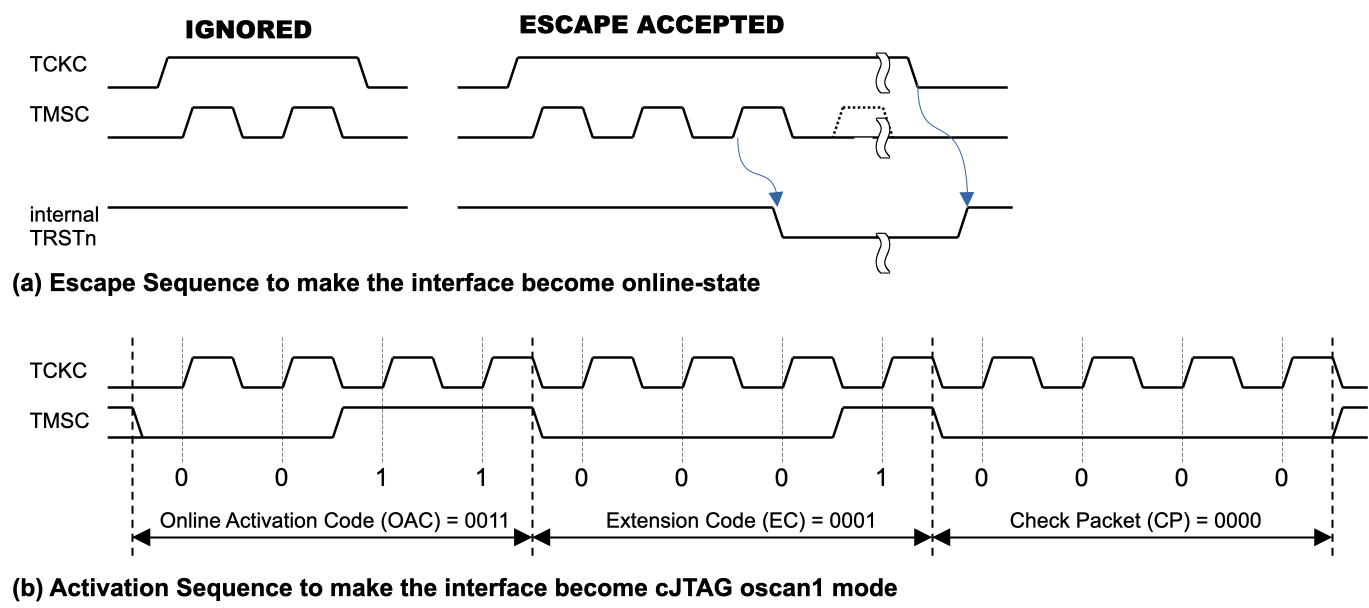
\includegraphics[width=1.00\columnwidth]{./Figure/cJTAG_ESC_ACT.png}
    \caption{cJTAG Escape Sequence and Activation Sequence}
    \label{fig:cJTAG_ESC_ACT}
\end{figure}

\begin{figure}[H]
    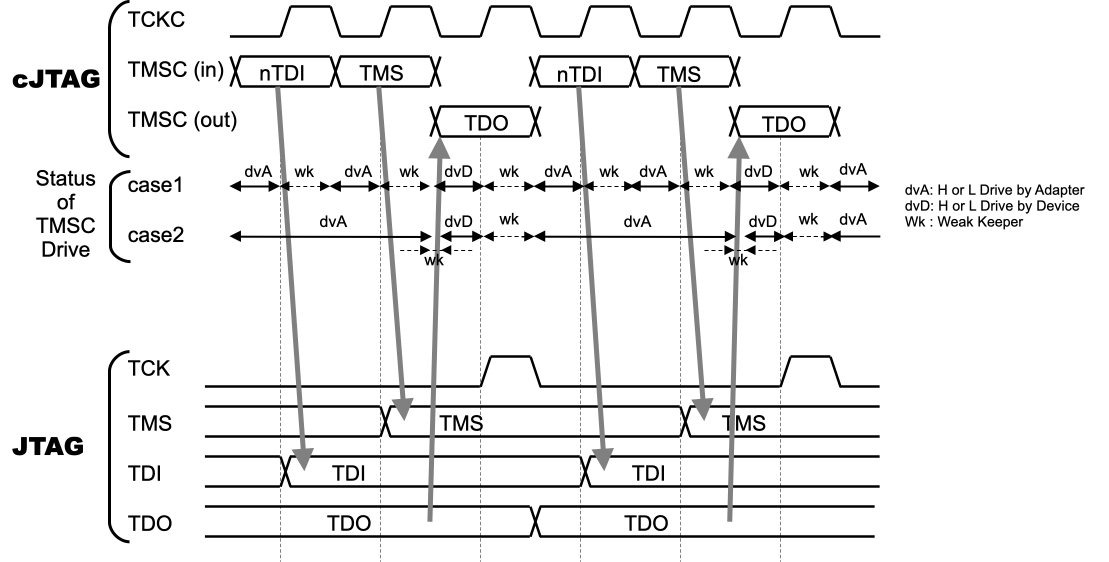
\includegraphics[width=1.00\columnwidth]{./Figure/cJTAG_OSCAN1.png}
    \caption{cJTAG OSCAN1 Sequence}
    \label{fig:cJTAG_OSCAN1}
\end{figure}

%=========================================================
% cJTAG TCKC/TMSC Pin Controls
%=========================================================
\subsection{cJTAG TCKC/TMSC Pin Controls}
\label{sec:cJTAG_PINCTRL}

To avoid a drive conflict in OSCAN1 Sequence, TMSC is driven by its source only while TCKC is low, and relies on a Bus Keeper logic to maintain a valid logic level while TCKC is high. Moreover, when the external adapter wants to start the escape sequence suddenly during the OSCAN1 sequence, especially during the CJTAG\_2\_JTAG is driving TMSC as TDO information, the CJTAG\_2\_JTAG should release TMSC by watching if the TCKC level is high.\\
As a result, the CJTAG\_2\_JTAG controls cJTAG pins as shown in Table \ref{tb:cJTAG_PINCONTROL} and the chip top block and I/O buffer block should follow this specification.\\

\begin{table}[hbtp]
    \begin{adjustbox}{scale={1.0}{1.0}}
    \textsf{
    \begin{tabular}{lllll}
        \hline
        %-----------------------------------
        \rowcolor{LightPurple}
        \textbf{Signal} &
        \textbf{Reset} &
        \textbf{Escape Sequence} &
        \textbf{Activation Sequence} &
        \textbf{OSCAN1 Sequence} \\
        \hline
        %-----------------------------------
        TCKC & Pull Up & Pull Up & Pull Up & Pull Up    \\
        TMSC & Pull Up & Pull Up & Pull Up & Bus Keeper \\
        \hline
        %-----------------------------------
  \end{tabular}
  }
  \end{adjustbox}
  \caption{cJTAG Pin Control}
  \label{tb:cJTAG_PINCONTROL}
\end{table}

%=========================================================
% cJTAG Halt on Rest
%=========================================================
\subsection{cJTAG Halt on Reset}

The CJTAG\_2\_JTAG supports the Halt-on-Reset function as well as the mmRISC-1 core does. As shown in Figure \ref{fig:cJTAG_HALT_ON_RESET}, when the negation of \seqsplit{RES\_ORG} occurs, if TMSC is driven at a high level, the CJTAG\_2\_JTAG does not assert \seqsplit{FORCE\_HALT\_ON\_RESET\_REQ}, and the CPU starts from the 1st instruction at reset vector, which is the normal operation. If TMSC is driven to a low level, the CJTAG\_2\_JTAG asserts \seqsplit{FORCE\_HALT\_ON\_RESET\_REQ}, and negates \seqsplit{FORCE\_HALT\_ON\_RESET\_REQ} after the assertion of \seqsplit{FORCE\_HALT\_ON\_RESET\_ACK} from the mmRISC core. Then the CPU halts before executing the 1st instruction at the reset vector until a resume command comes from debugger. During the time when the reset input is asserted, the TMSC should be pulled-up at the chip level as shown in Table \ref{tb:cJTAG_PINCONTROL}, so if TMSC is left open, the CPU starts execution normally.

\begin{figure}[H]
    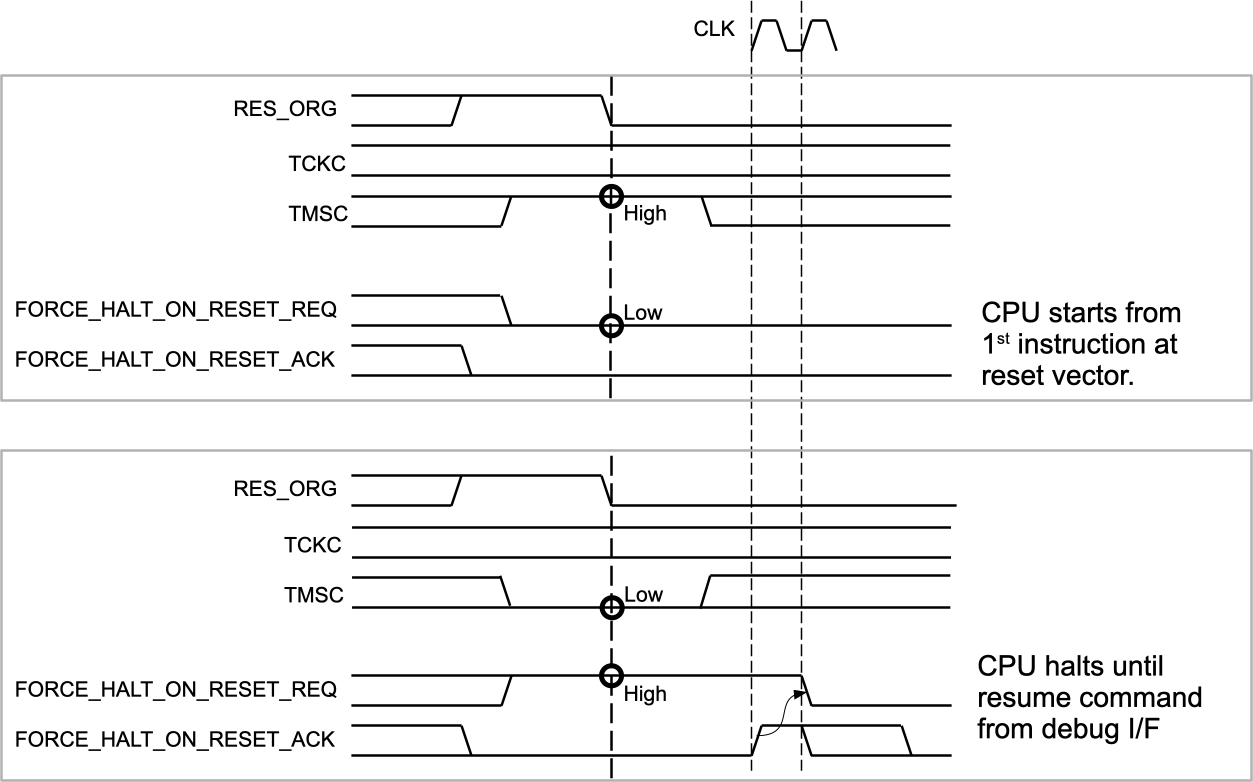
\includegraphics[width=0.9\columnwidth]{./Figure/cJTAG_HALT_ON_RESET.png}
    \caption{cJTAG Halt on Reset}
    \label{fig:cJTAG_HALT_ON_RESET}
\end{figure}

%=========================================================
% cJTAG Adapter (FTDI)
%=========================================================
\subsection{cJTAG Adapter (FTDI)}
\label{sec:cJTAG_ADAPTER}

In general, the interface adapter from USB to 4-wire JTAG for OpenOCD controlled by an FTDI chip is very popular. But if it is difficult for you to get an adapter from USB to 2-wire cJTAG which operates under the OpenOCD environment, you can make it by attaching a simple circuit (cjtag\_adapter.v) to the adapter from USB to 4-wire JTAG as shown in Figure \ref{fig:cJTAG_ADAPTER}. An example of a Verilog HDL code of the simple circuit (cjtag\_adapter.v) is shown in Listing \ref{list:cJTAG_ADAPTER}.\\

This simple circuit supports the Halt-on-Reset feature. If RESET\_HALT\_N (negative) is asserted to a low level at the negation of the reset input, TMSC goes to a low level to halt the CPU after reset. If you do not use the Halt-on-Reset feature of mmRISC-1, fix RESET\_HALT\_N to High.\\

Please note that this simple adapter does not follow the cJTAG standard because TMSC does not become HiZ during TCKC is high. But this adapter works fine even when connecting to cJTAG standard devices. During the OSCAN1 sequence of the cJTAG protocol, even if the adapter suddenly begins the escape sequence and the activation sequence, it drives TCKC to high and drives TMSC to high or low, there are no contentiona on TMSC signal because the target device does not drive TMSC due to TCKC's high level. \\
On the other hand, this adapter does not release TMSC when TCKC is high, which is a worry if there might be contention on TMSC line. As for the OpenOCD of RISC-V, during the TDO phase in the OSCAN1 sequence when the target device drives TMSC, the falling edge of TCK and the negating edge of TMS, both from JTAG adapter, are at the same time, which means TMSC becomes HiZ just at the falling edge of TCK. But the CJTAG\_2\_JTAG in the target device drives TMSC (as TDO) several clocks after the TCKC falling edge, and after the rising edge of TCKC (during TCKC is high), the target device releases TMSC, so this system can avoid signal contentions on TMSC line.

\begin{figure}[H]
    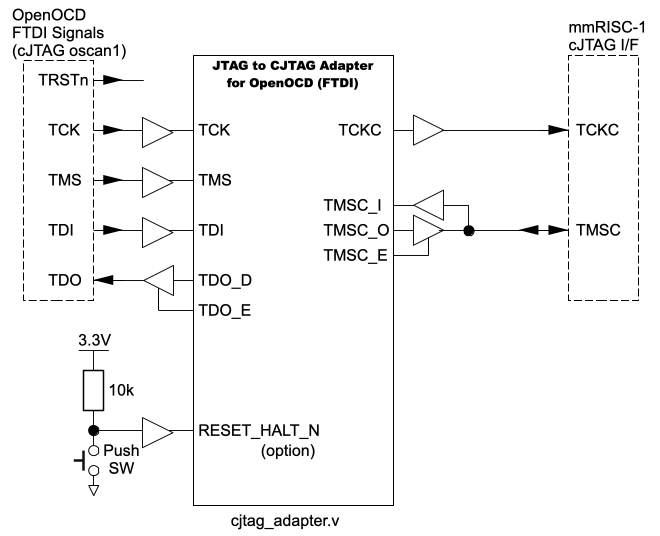
\includegraphics[width=0.8\columnwidth]{./Figure/cJTAG_ADAPTER.png}
    \caption{External Adapter to convert JTAG to cJTAG}
    \label{fig:cJTAG_ADAPTER}
\end{figure}

\begin{lstlisting}[caption=RTL code of cjtag\_adapter.v, label=list:cJTAG_ADAPTER, captionpos=b, language=Verilog, basicstyle=\ttfamily\scriptsize, frame=single]
// TCKC
// if Push SW is ON, Force High for target not to drive TMSC
// else Through TCK
assign TCKC   = (~RESET_HALT_N)? 1'b1
              : TCK;
// TMSC
// if Push SW is ON, Force Low to halt CPU
// else TMS determines output enable, 
//      and TDI determines output level
assign TMSC_O = (~RESET_HALT_N)? 1'b0
              : TDI;
assign TMSC_E = (~RESET_HALT_N)? 1'b1
              : (TMS          )? 1'b1
              :                  1'b0;
// TDO
assign TDO_D  = TMSC_I;
assign TDO_E  = 1'b1;
\end{lstlisting}

If you want to have a USB to cJTAG adapter which follows the standard specification of cJTAG, the adapter should watch the Escape sequence, the Activation sequence, and the OSCAN1 sequence. During the Escape sequence and the activation sequence, the driving state of TMSC is controlled by only TMS. Once entering OSCAN1 mode, the driving state of TMSC is controlled by not only TMS but also TCKC (HiZ during TCKC=1). This case can be realized by using some MCU device for the adapter. 

%=========================================================
% cJTAG Implementation for Silicon (SoC)
%=========================================================
\subsection{cJTAG Implementation for Silicon (SoC)}

An example of a cJTAG Implementation for Silicon (SoC) is shown in Figure \ref{fig:cJTAG_SoC}. At the same layer of mmRISC, a converter from cJTAG to JTAG (CJTAG\_2\_JTAG) is instantiated. The I/O buffer block including TCKC and TMSC should handle both the pull-up and the bus keeper function as described in Section \ref{sec:cJTAG_PINCTRL} which are supported by the CJTAG\_2\_JTAG block. The method to control the I/O Port for cJTAG Pins is shown in Listing \ref{list:cJTAG_IOCTRL}.

\begin{figure}[H]
    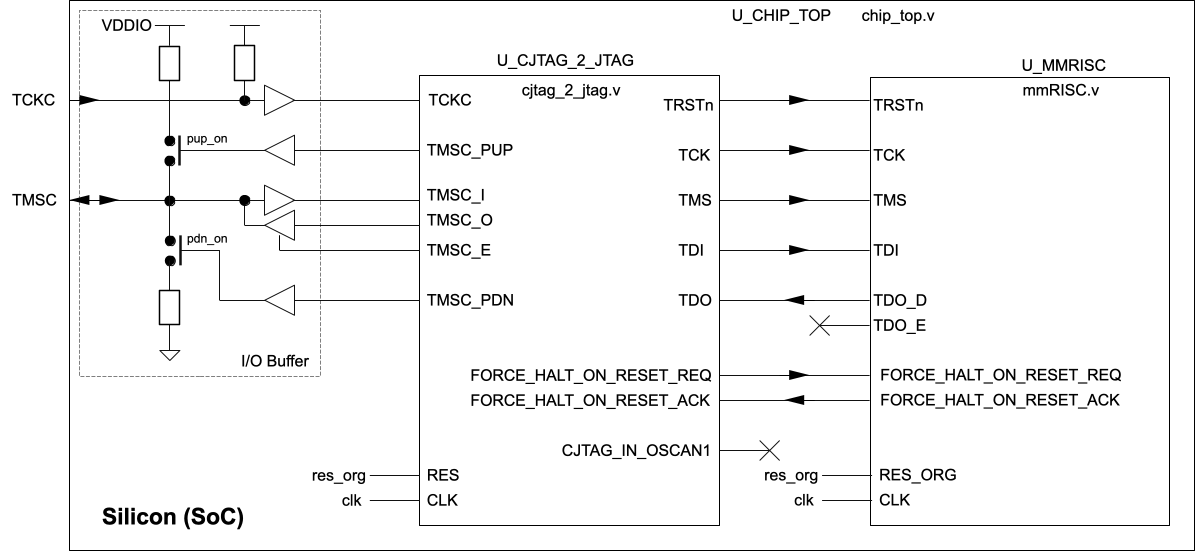
\includegraphics[width=1.00\columnwidth]{./Figure/cJTAG_SoC.png}
    \caption{cJTAG Implementation for Silicon (SoC)}
    \label{fig:cJTAG_SoC}
\end{figure}

\begin{lstlisting}[caption=I/O Port Control for cJTAG Pins, label=list:cJTAG_IOCTRL, captionpos=b, language=Verilog, basicstyle=\ttfamily\scriptsize, frame=single]
// During Reset , PULLUP ON, PULLDN OFF
// Before OSCAN1, PULLUP ON, PULLDN OFF
// During OSCAN1, Bus Keeper
//       (PULLUP when TMSC_I==1, PULLDN when TMSC_I==0)
// TMSC is driven only when in OSCAN1 mode.
//       (oscan1_state[2] shows it is in TDO phase.)
//
assign TMSC_PUP = ( RES            )? 1'b1
                : (~CJTAG_IN_OSCAN1)? 1'b1
                :   TMSC_I;
assign TMSC_PDN = ( RES            )? 1'b0
                : (~CJTAG_IN_OSCAN1)? 1'b0
                :  ~TMSC_I;
assign TMSC_E   = (RES )? 1'b0
                : (TCKC)? 1'b0
                : (CJTAG_IN_OSCAN1 & oscan1_state[2])? 1'b1
                : 1'b0;
\end{lstlisting}

%=========================================================
% cJTAG Implementation for FPGA and Test Bench
%=========================================================
\subsection{cJTAG Implementation for FPGA and Test Bench}
\label{sec:cJTAG_FPGA}


An example of a cJTAG Implementation for FPGA and Test Bench is shown in Figure \ref{fig:cJTAG_FPGA}. In this system, the CHIP\_TOP layer, which is the SoC top layer, is surrounded by an additional upper layer CHIP\_TOP\_WRAP.The cJTAG Adapter described in Section \ref{sec:cJTAG_ADAPTER} is located as CJTAG\_ADAPTER in the layer CHIP\_TOP\_WRAP. The cJTAG external pin controls described in Section \ref{sec:cJTAG_PINCTRL} are also performed in the layer CHIP\_TOP\_WRAP.\\

If you have a dedicated USB-cJTAG adapter, you can directly connect it to TCKC and TMSC of the SoC without loopback connections from U\_CJTAG\_ADAPTER in Figure \ref{fig:cJTAG_FPGA}.\\

If you want to realize a cJTAG Adapter which follows the cJTAG standard specification as described in the last paragraph of Section \ref{sec:cJTAG_ADAPTER}, the CJTAG\_ADAPTER block should watch the cJTAG protocol sequence like the CJTAG\_2\_JTAG block does.

\begin{figure}[H]
    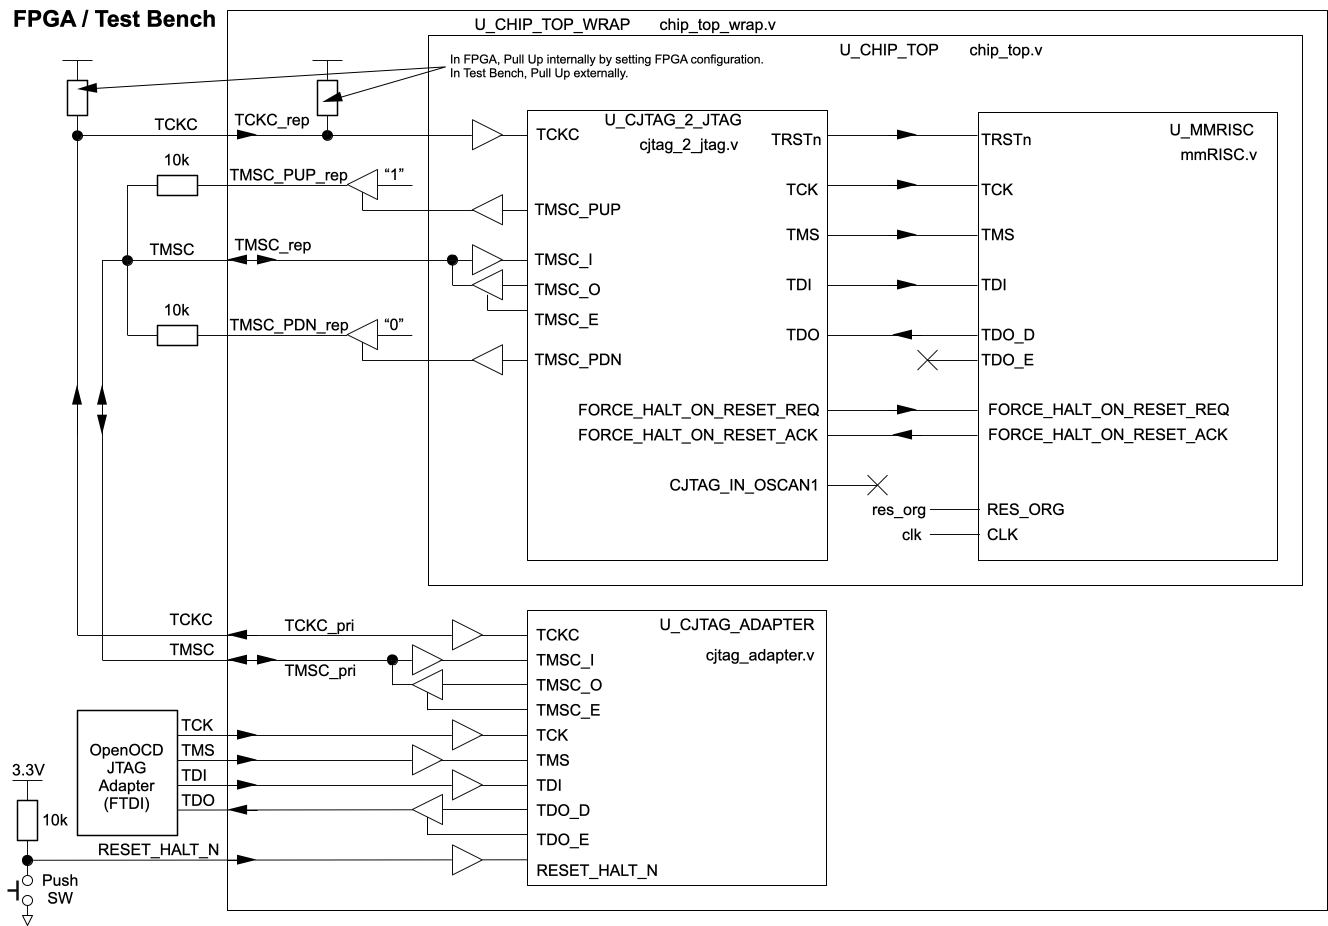
\includegraphics[width=0.90\columnwidth]{./Figure/cJTAG_FPGA.png}
    \caption{cJTAG Implementation for FPGA and Test Bench}
    \label{fig:cJTAG_FPGA}
\end{figure}






